\documentclass{article}
\usepackage[utf8]{inputenc}
\usepackage{amsmath}
\usepackage{graphicx}
\usepackage{hyperref}

\begin{document}
\title{Temperate Phage Modelling}
\author{Matthew So}
\maketitle

\section{Basic model}
These models have been developed in order to potentially address future questions about lysis-lysogeny decisions in temperate phages.
The more advanced models build upon this basic model. Detailed explanations for each term in the differentials and for each parameters can be found in the appropriate section in Section 2.

\subsection{State variables}
Explanations can be found in [2.1].
\begin{itemize}
\item $U$: Concentration of uninfected bacteria (bacteria/mL) 
\item $L$: Concentration of lysogens (bacteria/mL)
\item $P$: Concentration of phages (phages/mL)
\item $R$: Concentration of growth rate-limiting resource, assumed to be glucose.  (g/mL)
\end{itemize}

\subsection{Parameters}
\subsubsection{Regarding Monod growth} 
Explanations can be found in [2.2].
\begin{itemize}
\item $V_U$: maximum uninfected growth rate (1/hr)

\item $V_L$: maximum lysogen growth rate (1/hr)

\item $H$: concentration of resource resulting in half-maximal growth rate  (g/mL)

\item $e$: efficiency constant; amount of resource to create a new bacterium (g/bacterium)
\end{itemize}

\subsubsection{Regarding death rates} 
Explanations can be found in [2.3].
\begin{itemize}
\item $D_b$: maximal bacterial death rate (/hr)

\item $\eta$: reciprocal of the concentration of resource resulting in half-maximal death rate. (mL/g)
\end{itemize}

\subsubsection{Regarding any phages} 
Explanations can be found in [2.4].
\begin{itemize}
\item $\beta$: burst size (unitless)
\item $K_a$: adsorption constant (mL/phages/hr)
\item $D_p$: destruction rate of free phage (/hr)
\end{itemize}

\subsubsection{Regarding temperate phages} 
Explanations can be found in [2.5].

\begin{itemize}
\item $\phi$: probability of lysogeny upon infection (unitless)

\item $r$: induction rate, the probability of any lysogen to induce lytic cycle during a time period dt. (/hr)
\end{itemize}
\subsubsection{Regarding ecosystem maintenance} 
Explanations can be found in [2.6].
\begin{itemize}
\item $d$: dilution rate (/hr)

\item $i$: infusion rate (g/mL/hr)
\end{itemize}


\subsection{Differentials}

$
m(R, H) = \underbrace{\frac{R}{R+H}}_{\text{Proportion of maximal growth rate [2.2]}} \\ \\
q(R, \eta) = \underbrace{\frac{1}{R\eta+1}}_{\text{Proportion of maximal death rate [2.3]}}\\ \\
N_U = \underbrace{V_U \cdot U \cdot m(R, H)}_{\text{Uninfected growth [2.2]}} \\ \\
N_L =  \underbrace{V_L \cdot L \cdot m(R, H)}_{\text{Lysogen growth [2.2]}} \\ \\
I_{Lyso} = \underbrace{\phi \cdot K_a \cdot P \cdot U}_{\text{new infections choosing lysogeny [2.5]]}}\\ \\ 
I_{lyt}= \underbrace{(1- \phi) \cdot K_a \cdot P \cdot U}_{\text{new infections choosing lytic cycle [2.4/2.5]}}  \\ \\ \\ 
\frac{dU}{dt} = \underbrace{N_U}_{\text{Uninfected growth [2.2]}} - \underbrace{D_b \cdot U \cdot q(R, \eta)}_{\text{Uninfected bacterial deaths [2.3]}} \\ \\ - \underbrace{K_a \cdot P \cdot U}_{\text{New phage adsorptions [2.4]}} - \underbrace{d \cdot U}_{\text{dilution [2.6]}} \\ \\
\frac{dL}{dt} = \underbrace{N_L}_{\text{Lysogen growth [2.2]}}+ \underbrace{I_{Lyso}}_{\text{Lysogenic cycle chosen upon infection [2.5]}} - \underbrace{D_b \cdot L \cdot q(R, \eta)}_{\text{Lysogen deaths [2.3]}} \\ \\ - \underbrace{r \cdot L}_{\text{Inductions [2.5]}} - \underbrace{d \cdot L}_{\text{dilution [2.6]}} \\ \\
\frac{dP}{dt} = \underbrace{\beta \cdot r \cdot L}_{\text{Released from induction [2.5]}}  + \underbrace{\beta \cdot I_{lyt}}_{\text{Released from lytic cycle choice [2.4/2.5]}} \\ \\ - \underbrace{K_a \cdot P \cdot (U+L)}_{\text{Lost to adsorption [2.4]}} - \underbrace{D_p \cdot P}_{\text{Destruction of free phage [2.4]}} -\underbrace{d \cdot P}_{\text{dilution [2.6]}}\\ \\
\frac{dR}{dt} = \underbrace{-e \cdot (N_U + N_L)}_{\text{Use of resource to grow new bacteria [2.2]}} + \underbrace{i}_{\text{Infusion of new resource [2.6]}} - \underbrace{d \cdot R}_{\text{dilution [2.6]}} \\ \\
$

\section{Model-building explanations}
 These models consider a well-mixed system of bacteria and phage in an environment with some concentration of resources.

\subsection{First Choices of State Variables}
A system to model lysis-lysogeny decisions would not be possible without phages, as well as their bacterial hosts. Since the lysogenic cycle can convert uninfected bacteria to lysogens, both these variables must be tracked as well. Additionally, I use a resource-dependent model of bacterial growth, in part to explore conditions of cyclic resources (which are important in the ecology of temperate phages). In this case, I assumed that the limiting resource was energy (glucose), as this was the only resource I could find data for. 

I assume lysogens and uninfected bacteria to have similar laws governing their growth and phage adsorption unless otherwise stated.

\subsection{Modelling resource-dependent bacterial growth}
There exist many models of bacterial growth, but all choices of models should include the following:

Bacterial growth rates should be a monotonically increasing function of resources. ($\frac{dB}{dR} \geq 0$). This is because bacteria grow more slowly when there are fewer resources available for their growth. 

There should exist a maximal bacterial growth rate ($V$), which is achieved when resource levels are high. (as $R \rightarrow \infty,  \frac{dB}{dR} \rightarrow V$). This is because the rate of bacterial growth cannot increase indefinitely as extracellular resources increase.

Bacterial resource utilization should increase as the bacterial growth rate increases. This is because the resources for bacterial growth are derived from the environment.

One growth function satisfying these assumptions is the empirically derived Monod bacterial growth function (Cunningham et al., 2010). 

\begin{center} $
m(R, H) = \frac{R}{R+H}$

$
\frac{dB}{dt} = V \cdot m(R, H) \cdot B$

$\frac{dR}{dt} = -e \cdot V \cdot m(R, H) \cdot B $
\end{center}

Firstly, I observed the form of $m$. This function is concave down, is bounded between 0 and 1, and is equal to 0 when $R=0$. 

Looking at $\frac{dB}{dt}$, it is clear that this function represents the proportion of the maximal growth rate achieved at a given resource concentration. It also incorporates the maximal growth rate which was discussed earlier. 

Next, I observed the form of $\frac{dR}{dt}$. This differential makes the resource utilization equal to the number of new bacteria, multiplied by $e$. Therefore, $e$ represents the amount of resources used to form a new bacterium. However, this means that the model does not capture any baseline resource utilization by bacteria independent of bacterial growth; this was omitted for stability considerations.
 
If given an initial amount of resource, the growth function produces a sigmoid-shaped bacterial growth curve with respect to time, which is expected. However, this population saturation is due to the growth rate vanishing to zero as resources are used. In general, the Monod model cannot capture bacterial death.

\subsection{Bacterial death}
Bacteria should have a natural death rate, which monotonically decreases with the resource concentration. In an ecosystem, bacteria can die in many ways unrelated to phages, but it is likely that resource deprivation would decrease this rate of death as they would be less likely to be able to adapt to their environment with low energy. 

A convenient function for a bacterial death function related to resource deprivation might be related to bacterial growth in the Monod growth function, due to the link between bacterial death and resource concentration. However, instead of the growth rate increasing with increased resource, we have the death rate decreasing with increased resource.

We would like to represent the proportion of the maximal death rate achieved with 1-m (as this is bounded between 0 and 1, and decreases the death rate with increasing resource). However, we may reformulate this death equation to assume constant rates of bacterial death if required.

\begin{center}
\begin {equation} 
\begin{split}
q(R, H) = 1-m(R, H)) \\ \\ q(R, H) = 1 - \frac{R}{R+H}\\ \\  q(x, H) = \frac{H}{R+H} \\ \\ \eta = \frac{1}{H} \\ \\ q(x, \eta) = \frac{\frac{1}{\eta}}{x+\frac{1}{\eta}} \\ \\ q(R, \eta) = \frac{\frac{1}{\eta}}{\frac{R\eta + 1}{\eta}} \\ \\ q(R, \eta) = \frac{1}{R\eta + 1} 
\end{split}
\end {equation}
\end{center}

As $H \rightarrow \infty, \eta \rightarrow 0$. If $\eta=0$, $q(x, \eta) = 1$, leading to a constant rate of bacterial death. 

\subsection{Adding simple phages}
Phage-bacteria binding should follow the law of mass action, as the binding between phages and bacteria is a chemical process (Storms $\&$ Sauvageau, 2015). Briefly, this states that the binding rate should be directly proportional to both the phage concentration and the bacterial concentration, and assumes that phages and bacteria are interacting due to chance.

This model assumes that each adsorption to an uninfected bacterium leads to an infection, with no failed infections. This is unrealistic (for example, restriction enzyme systems may lead to failed infections, among others), but has been left out for simplicity. However, one could model this by assuming a constant or changing rate of infection failure. Additionally, phages adsorbed in this way are removed from the free phage compartment. 

I assume that free phages are degraded at a constant rate independent of adsorption to bacteria. For example, they may be adsorbed to other things in the environment, or by exposure to UV radiation. 

The model also assumes that bacteria entering the lytic cycle instantly die, producing a constant number of phages. These are both unrealistic assumptions made for the sake of simplicity. The lytic cycle takes time to produce phages and to lyse the cell, and the number of phages produced per bacterium is not constant (	Delbrück, 1945). The number of phages produced per bacterium is modeled as the average burst size. In reality, the number of phages produced likely depends on how many phages can be made before the cell lyses due to lysis-inducing protein production, which depends on how readily bacterial resources can be mobilized. 

\subsection{Adding temperate dynamics}

Upon infecting an uninfected bacterium, phages choose between lysis and lysogeny (Gandon, 2016). Thus, a bacterium infected by a lysogeny-choosing phage will become a lysogen. There is evidence to suggest that this is true; this choice can be modeled in several ways described later. However, as a simple model, one could model this as a constant probability of lysogeny upon infection. 

Phages may adsorb to lysogens at a similar rate compared to uninfected bacteria, but phage adsorptions to lysogens do not lead to lysis. This assumption may be realistic for some kinds of superinfection inhibition, but not others. In phage $\lambda$, the mechanism of superinfection inhibition is the binding of a repressor protein (associated with lysogeny) to the virulence-controlling operator (Gandon, 2016). Therefore, phages may freely enter the cell, but the lysogenic state will be retained (as the repressor proteins will already exist inside of a lysogenic bacterium). However, in some other phages, superinfection resistance may be due to removing receptors allowing for other phages to enter, which would lead to different mechanics. 

Lysogens may spontaneously induce a lytic cycle. Most literature shows that lysogens have a low spontaneous induction rate, which may be incorporated into a simple model (Gandon, 2016). However, it has also been shown that induction rates decrease during starvation and increase due to DNA damage, but this will not be explored for simplicity.

\subsection{Ecosystem maintenance}

I assume that the ecosystem is maintained by a constant infusion of resources. In some cases, this might be true (for example, if the rate-limiting resource is glucose derived from energy obtained from sunlight). This is a fairly simple assumption that may be realistic. 

Each free component of the ecosystem may be subject to dilution over time. This has been done in microbiology to model bacteria growing in a chemostat (Ziv et al., 2013). However, this might also be realistic in other ecosystems where dilution may occur, for example, marine ecosystems. 

\subsection{Parameter Sampling}

All parameters which were not arbitrarily set are sampled from a log-uniform distribution (random variable with logarithm that is uniformly distributed). The mean of this distribution is set to the mean of the logarithms of upper and lower bounds found in the literature, while the standard deviation of the distribution is set to the (upper bound - mean)/2, meaning that the parameter falls between the two bounds 95$\%$ of the time. This method ensures that the probability density function is continuous, unlike the uniform distribution, while still only allowing the sampling of non-negative parameters. Additionally, it allows exploration of parameters whose upper and lower bounds are different by several orders of magnitude. However, the arbitrary choice of the mean for the log-uniform distribution from the upper and lower bounds may be incorrect.

\section{Modifications to the basic model}
\subsection{Multiplicity of infection}
\subsubsection{Intuition}
The probability of lysogeny in phage $\lambda$ is known to increase when the bacterium is infected by multiple phages at once (Zeng et al., 2010). One reasonable assumption to model this is that the number of phages infecting a bacterium is Poisson distributed with mean equal to $K_aP$ (Figliozzi et al., 2016). This way, the interpretation of the Poisson distribution is the probability that one given bacteria will be infected with N coinfecting phages. Additionally, we will require a function mapping the number of coinfecting phages to a probability of lysogeny.

\subsubsection{Model building}
For this MOI model, a time scale important to viral replication must be used. Therefore, I chose a time scale equal to 1/10th of the lysis time of phage $\lambda$, equal to 4.5 minutes (Ryan $\&$ Rutenberg, 2007). This selection of 1/10th of the lysis time has been used in other modelling studies (Mitarai et al., 2016). 

$\pi(N)$: The probability of lysogeny as a function of the number of coinfecting phages. 

\begin{center}$
p(\lambda, N) = \underbrace{\frac{{e^{ - \lambda } \lambda ^N}}{{N!}}}_{\text{pdf of Poisson distribution}}$
$\lambda = \underbrace{K_a \cdot P}_{\text{mean of the Poisson distribution}}$
\end{center} 

Firstly, we can compute the probability that any one bacterium will become lysogenized:
\begin{center}
$=\sum_{N=1}^{\infty}{p(\lambda, N) \cdot \pi(N)}$
\end{center}

However, what we want is actually the probability that any \emph{infected} bacterium will become lysogenized. To get this, we will divide this term by the total infection probability. 
\begin{center}
$
\phi = \underbrace{\frac{\sum_{N=1}^{\infty}{p(\lambda, N) \cdot \pi(N)}}{\sum_{N=1}^{\infty}p(\lambda, N) }}_{\text{probability of lysogeny given infection}}$
\end{center}

which is equivalent to 
\begin{center}
$\phi = \underbrace{\frac{\sum_{N=1}^{\infty}{p(\lambda, N) \cdot \pi(N)}}{1-p(\lambda, 0)}}_{\text{probability of lysogeny given infection}}$
\end{center}

However, one question remains: What is the form of $\pi(N)$? Fortunately, the literature suggests that the form is a Hill function, therefore following the following form suggested by Zeng et al.

\begin{center}
$\pi(N) = \frac{Nh}{Nh + Kh}$
\end{center}

 

The Poisson distribution theoretically allows for any number of coinfecting phages, but the impact of larger numbers of coinfecting phages becomes vanishingly small and may be ignored. In practice, we calculate each summation term up to N=20. This new $\phi$ can be used in place of the original parameter $\phi$ in the basic model.

\subsection{Quorum sensing}
\subsubsection{Intuition}
A quorum-sensing system has been found to increase the probability of lysogeny in phages using this system in the presence of the quorum-sensing (arbitrium) peptide (Erez et al., 2017). 
The probability of lysogeny should be a monotonically increasing function of arbitrium concentration, and is therefore bounded between 0 and 1. Binding of the arbitrium receptor leads to the downregulation of an operator favoring lytic activity, so from a biological standpoint, it seems unlikely that increasing arbitrium would actually decrease lysogenic activity at any point. A convenient function here might be yet another Monod-type function for simplicity, as the exact functional form of the system is not yet known. 

I also assume that there is a baseline probability of lysogeny independent of arbitrium concentration. This is supported by the paper. This lends itself to a functional form equal to a constant baseline, plus some monotonically increasing function of arbitrium (due to the activation of the arbitrium system).

Another assumption is that produces a constant (the average) number of arbitrium peptides upon lysogenic infection. This is likely unrealistic, but done for simplicity. I also assume that the arbitrium peptides have a constant rate of degradation, as the peptides cannot accumulate forever. 

\subsubsection{Model building}
Firstly, we will track a new state variable $A$, the concentration of the peptide in the system (peptides/mL). The probability of lysogeny should be of the form

\begin{center}
$ \phi = \underbrace{\phi_0 + f(A) \cdot (1-\phi_0)}_{\text{sum of lysogeny probability due to baseline and arbitrium}}$
\end{center}

where $\phi_0$ represents the baseline level of lysogeny. $f(A)$ should be a monotonically increasing function bounded between 0 and 1, so this term is scaled by $(1-\phi_0)$ to ensure that the total probability of lysogeny remains between 0 and 1.

Unlike for the MOI model, the literature does not have any data on the functional form of $f(A)$. For convenience, I will choose the simple form 

\begin{center}
$f(A) = \frac{A}{H_A+A}$
\end{center}

where $H_A$ represents the arbitrium concentration resulting in half-maximal increase in probability of lysogeny due to the arbitrium system.

The arbitrium peptides are produced in some quantity $n_A$ upon all phage infections, degrade at a constant rate $d_A$, and are diluted at a constant rate $d$. Therefore, 
\begin{center}
$\frac{dA}{dt} = \underbrace{n_AK_aPU}_{\text{production of peptide due to infection}}-\underbrace{D_AA}_{\text{degradation of peptide}}-\underbrace{d \cdot A}_{\text{dilution}}$
\end{center}

The basic model may be modified by tracking $A$, adding this differential, and adding $f(A)$ from this modification to the original constant $\phi$ (which would now be called $\phi_0$). However, there does not seem to be enough data in the literature to estimate many important parts of this system (confirming a form for f(A), estimating $H_A$ if applicable, $n_A$, and $D_A$), so estimating applicable parameters and testing the model will have to be left as a future endeavor. 

\section{Initial conditions and parameter choices}

\subsection{Initial conditions for state variables}
\begin{itemize}
\item $U_0$: 1 bacteria/mL. I arbitrarily set a low bacterial concentration so that the entire growth curve could be observed.
\item $L_0$: 0 bacteria/mL. I assumed that no bacteria were infected at time 0.
\item $P_0$: 1 bacteria/mL. Often, in laboratory experiments, bacteria are infected with a multiplicity of infection of 1 (in this context, MOI means the ratio of viral concentration to bacterial concentration, not the number of coinfecting phages). 
\item $R_0$: Arbitrarily set equal to infusion rate. 
\end{itemize}

\subsection{Parameters regarding Monod growth}

\begin{itemize}
\item $V_U$: 0.5-10 (1/hr). Biological range used by Sinha et al., 2017. 

\item $V_L$: Set to $V_U/2$ (significantly slower than $V_U$).

\item $H$:$15 \times 10^{-9} - 35 \times 10^{-9}$ (g/mL). Upper bound is the $K_s$ for \textit{Escherichia coli}, while lower bound is the $K_s$ for \textit{Chelatobacter heintzii}. (Füchslin et al., 2011)

\item $e$: $5.98\times 10^{-13} - 5.4 \times 10^{-12}$ g/bacterium. Lower bound from estimate that $2 \times 10^9$ molecules of glucose required per cell (Phillips $\&$ Milo, 2009).  Upper bound from estimate that $1.8 \times 10^10$ molecules of glucose required per cell (Allen $\&$ Waclaw, 2018). 
\end{itemize}

\subsection{Parameters regarding death rates}
\begin{itemize}
\item $D_b$: $1 \times 10^{-4} - 1 \times 10^{-2}$ /hr. Arbitrarily set.

\item $\eta$: 0 mL/g. Set to allow constant bacterial death rates, allowing for analysis as described in section 5.
\end{itemize}

\subsection{Regarding any phages}
\begin{itemize}
\item $\beta$: 20-1000 (unitless). Biological range used by Sinha et al., 2017. 
\item $K_a$: $4.46 \times 10^{-9} - 6.18 \times 10^{-7}$ (mL/phages/hr). Estimates from lowest and highest adsorption rates used by Gallet et al., 2009.
\item $D_p$: $1 \times 10^{-7}$ (/hr). Arbitrarily set as a low number as literature suggests free phage death rate is low.
\end{itemize}

\subsection{Regarding temperate phages}
\begin{itemize}
\item $\phi$: 1 \times $10^{-5} - 0.35$ (unitless). Upper bound adapted from range from fitting from Sinha et al., 2017, lower bound set as a number close to 0 (following the lower bound of the same range). 

\item $r$: $1 \times 10^{-4} - 1 \times 10^{-3}$. (/hr). Lower bound suggested by Gandon, 2016 as a low induction rate, upper bound suggested as a high induction rate. 
\end{itemize}

\subsection{Regarding ecosystem maintenance}
\begin{itemize}
\item $d$: 0 (/hr). Various dilution rates explored initially, but in the end, set to 0 to allow for section 5 analysis.

\item $i$: $4.8 \times 10^{-10} - 4.8 \times 10^{-9}$ (g/mL/hr). Upper limit taken from estimate of glucose flux from other studies cited in (Hanson $\&$ Snyder, 1979). Lower limit set as an order of magnitude lower than upper limit, taking into account that the study authors found that the estimate of glucose flux was likely to overestimate the true value.
\end{itemize}

\subsection{Regarding the multiplicity of infection model}
\begin{itemize}
\item $h$: 1.00 (unitless). Determined by Zeng et al.
\item $K$: 1.812 (unitless). Estimated from Figure 2C in the paper published by Zeng et al. in 2010, with h fixed at 1.00. Unfortunately, even though the authors determined the value of K, the authors do not give its value.
\item Lysis time: 0.75 hr, for the $\lambda$ - \textit{E. coli} system. (Ryan $\&$ Rutenberg, 2007)
\end{itemize}

\section {Equilibrium estimates}
We can obtain upper or lower bounds for model equilibria by making assumptions, setting differentials to 0, and solving the resulting system of equations. Some of these estimates are actually exact values for model equilibria.

\subsection{Bacteria with no phages}
The equations governing bacterial growth in the absence of phage and with constant bacterial death are:

\begin{equation}
\begin{split}
\frac{dU}{dt} = V_UU\frac{R}{R+H} - D_BU - d \cdot U \\
\frac{dR}{dt} = -eV_UU\frac{R}{R+H}  - d \cdot R \\
\end{split}
\end{equation}

At equilibrium, there is no change in the bacterial concentration or the resource concentration. At equilibrium, there is also no change in the resource concentration. Since this is a system of two equations, we can solve for U and R. 

\begin{equation}
\begin{split}
0 = V_UU\frac{R}{R+H} - D_BU - d \cdot U \\
0 = -eV_UU\frac{R}{R+H}  - d \cdot R \\
\end{split}
\end{equation}

I used Maple (a mathematical software) to solve these equations, and the solutions were:

\begin{equation}
\begin{split}
R = \frac{HD_B}{V - D_B}, \\ U = \frac{i}{eD_B}
\end{split}
\end{equation}

These are surprising results, as the maximal bacterial growth rate counterintuitively does not contribute to the final carrying capacity of the model, and the infusion rate does not contribute to the final resource concentration (due to supporting a higher bacterial population). Notice that neither equilibrium R nor U are affected by initial conditions. The Monod law, in contrast, does predict that equilibrium U is affected by initial conditions (intuitively, in the Monod law, the equilibrium is $U = R_0/e$ as all resources are converted to bacteria, with no loss from bacterial death). 

(With dilution, a simplified result is also possible but the results are significantly messier; dilution will not be considered for subsequent analyses). 

\subsection{Bacteria with phages}
The equations governing bacterial growth in the presence of phage and with constant bacterial death are listed in section 1.3. Similarly, if we set all the differentials to 0 ($
\frac{dU}{dt} = 0, \frac{dR}{dt} = 0, \frac{dL}{dt} = 0, \frac{dP}{dt} = 0
$), we can obtain analytic solutions for the system equilibrium. However, while solvable, the solutions are unintelligible.  

One simplifying assumption is that at the end of a successful infection, nearly all of the phages are produced by induction. Thus, $\frac{dP}{dt} = \beta r L - K_a P L$. Using this assumption, we can obtain some bounds on equilibrium concentrations by assuming that U=0. After solving all of the differentials, we obtain:

\begin{equation}
\begin{split}
P = \frac{i \beta r }{K_a i + D_p e (D_B+r)} \\ \\
R = \frac{-H (D_B + r)}{D_B - V_L + r} \\ \\
L = \frac{i}{e (D_B + r)}
\end{split}
\end{equation}

Unsurprisingly, the higher the induction rate and burst size, the more free phages at equilibrium. One less obvious point is that the phage concentration at equilibrium decreases with increasing $K_a$, which is because lysing more uninfected bacteria is less important than being adsorbed into existing lysogens. For the lysogens, we find that the equilibrium is hardly different from the case with no phages, which makes sense as the lysogens are unaffected by external phage (dying slightly more frequently due to $r$).

The phage prediction puts a lower bound on the number of phages at equilibrium (as phages can also be produced through lysing uninfected bacteria). The resource prediction puts an upper bound on the amount of resources at equilibrium (as uninfected bacteria utilize resources to grow). The lysogen prediction puts a lower bound on the number of lysogens at equilibrium, as lysogens may also be produced by infecting uninfected bacteria. In practice, the estimate for phages is quite accurate, while R and L estimates are on the same order of magnitude of the actual R and L. However, the accuracy of the estimates decrease with increasing $D_p$.

From the phage and lysogen estimates, assuming the entire bacterial population consists of lysogens, the VMR (ratio of free phage to bacteria) can be estimated as 
\begin{center}
\begin{align*}
P = \frac{i \beta r }{K_a i + D_p e (D_B+r)} \\ \\
L = \frac{i}{e (D_B + r)} \\ \\
\text{VMR} = \frac{P}{L} \\ \\
\text{VMR} = \frac{\frac{i \beta r }{K_a i + D_p e (D_B+r)}}{\frac{i}{e (D_B + r)}} \\ \\
\text{VMR} = \frac{\beta r e (D_B + r)}{K_a i + D_pe (D_B + r)}
\end{align*}
\end{center}

Unsurprisingly, VMR is increased with increased burst size and induction rate (more free phage).

\subsection{Resource shocks}
Due to having growth mechanics borrowed from the Monod law, the peak of the bacterial curve resulting from a sudden infusion of resource must be lower than the $R$ after the shock, divided by $e$. However, the exact height of the peak will depend on the rate of resource utilization at the time of the shock (which depends on $V, H$, and $R$), as well as factors which can kill the bacteria such as phage and bacterial death rate. 

However, as stated before, short-term resource shocks do not affect the long-term equilibrium in this model. In real life, it is probably possible for a resource shock to completely wipe out all bacteria and phage in a system, leading to an equilibrium of 0 even after resources return; however, all concentrations in this model asymptotically approach 0, leading to an inevitable return of the populations if resources return. 

\section{Results from model integration}
\subsection {Bacteria without phage}

\subsubsection{Equilibrium}
\begin{center}
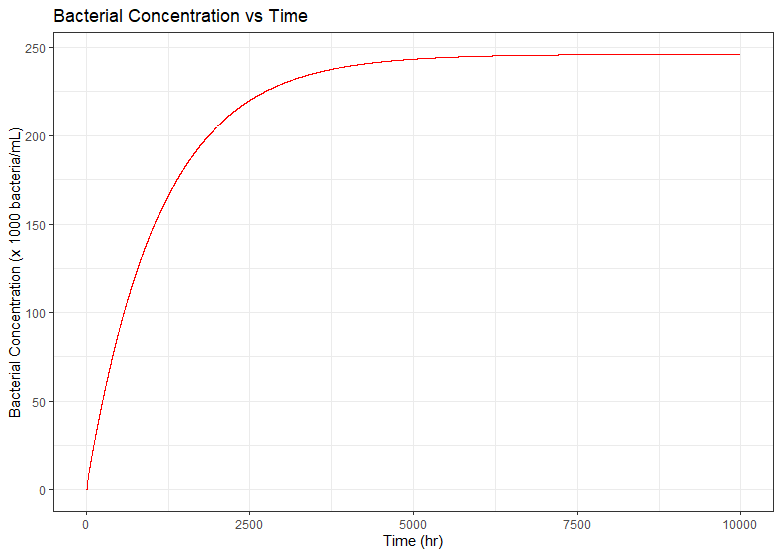
\includegraphics[scale=0.5]{plots/NoPhage_U.png}

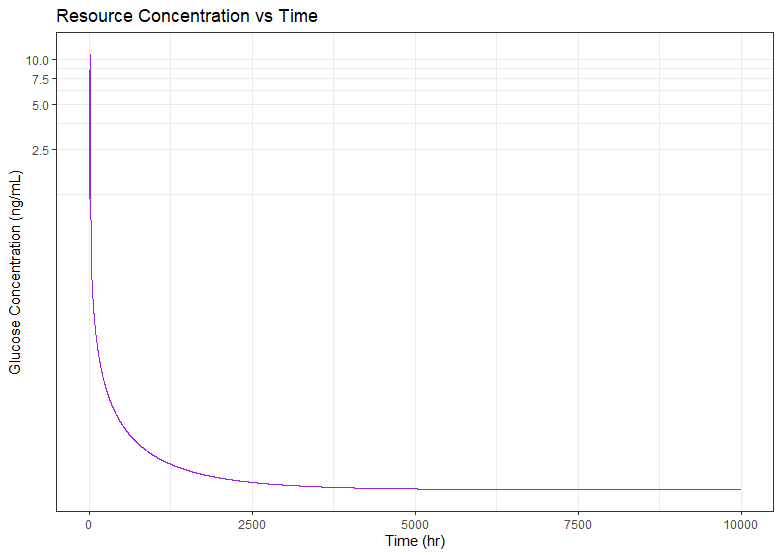
\includegraphics[scale=0.5]{plots/NoPhage_R.png}

\end{center}

These plots are representative examples of the saturating Monod-type growth exhibited by this model. (The resource plot has a log-scaled y axis) Saturation usually takes between $10^3$ to $10^4$ hours to complete at the resource concentrations in this model. 

As mentioned in section 4.1, the equilibrium resource and bacterial concentrations can be determined from the following equations:

\begin{equation}
\begin{split}
R = \frac{HD_B}{V - D_B}, \\ U = \frac{i}{eD_B}
\end{split}
\end{equation}

For example, after 10000 hours, the bacterial concentration is 245.9 x1000 bacteria/mL and the resource concentration is 0.01283 ng/mL. This is equal to the theoretical concentrations predicted by the previous equations to 4 significant digits.

\subsubsection{Initial growth}
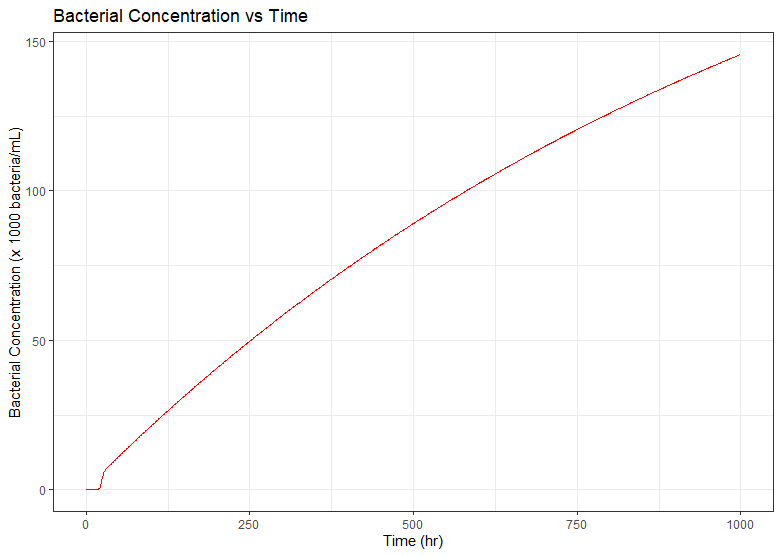
\includegraphics[scale=0.5]{plots/NoPhage_U_zoomed.png}

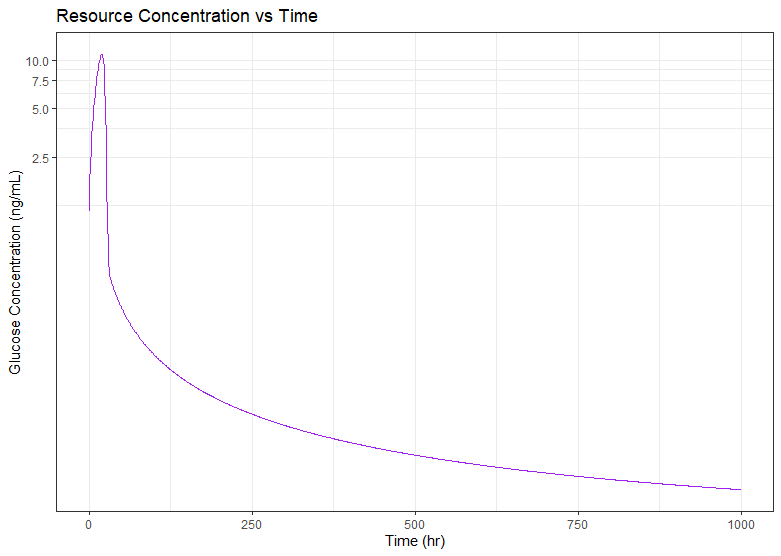
\includegraphics[scale=0.5]{plots/NoPhage_R_zoomed.png}

Resources typically increase for the first part of the curve due to the constant infusion rate (and low bacterial utilization), reach a peak, then level off. While the resource concentration is increasing, the bacterial concentration is concave up (as $\frac{R}{R+H}$ in $\frac{dR}{dt}$ increases with increased R), and the rest of the graph is concave down for analogous reasons. 

\begin{center}
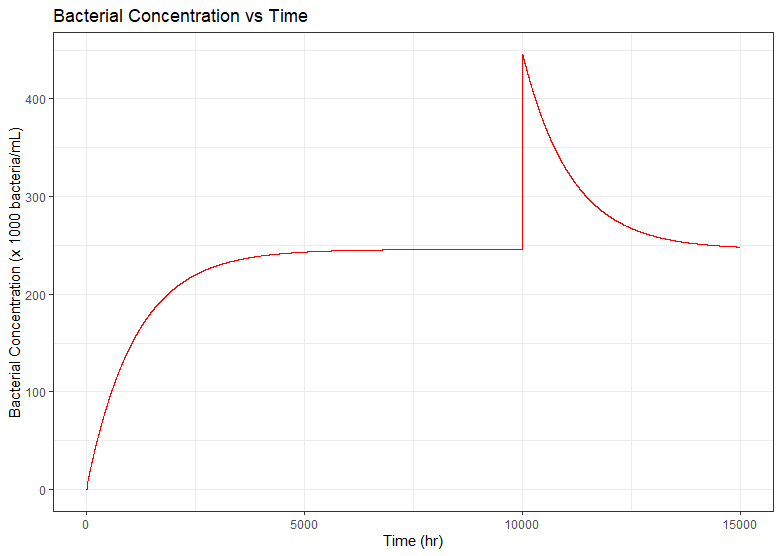
\includegraphics[scale=0.5]{plots/NoPhage_U_perturbed.png}

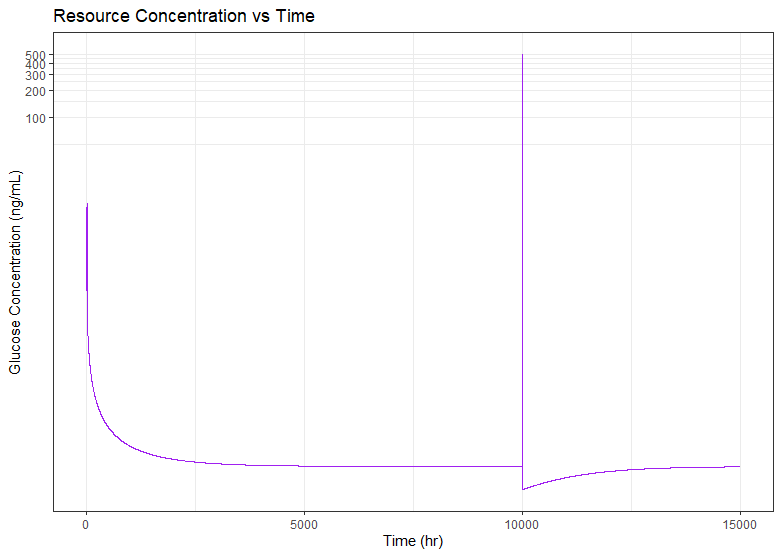
\includegraphics[scale=0.5]{plots/NoPhage_R_perturbed.png}
\end{center}

\subsubsection{Perturbation: increase in resources}
The model also reacts to perturbations. In this example, I have increased the resource level by 500 ng/mL at t=10000. This should theoretically temporarily increase the bacterial population by (500 ng/mL)/$e$, which is about 200 $\times$ 1000 bacteria/mL. This increase of 200 $\times$ 1000 bacteria/mL is reflected in the peak of the bacterial concentration graph, which is about 200 units higher than it was at t=10000. This increased resource utilization due to a higher population to causes the glucose concentration to temporarily fall below the normal equilibrium, but bacteria die until the carrying capacity is achieved once again. 

\begin{center}
\subsubsection{Perturbation: decrease in infusion rate}

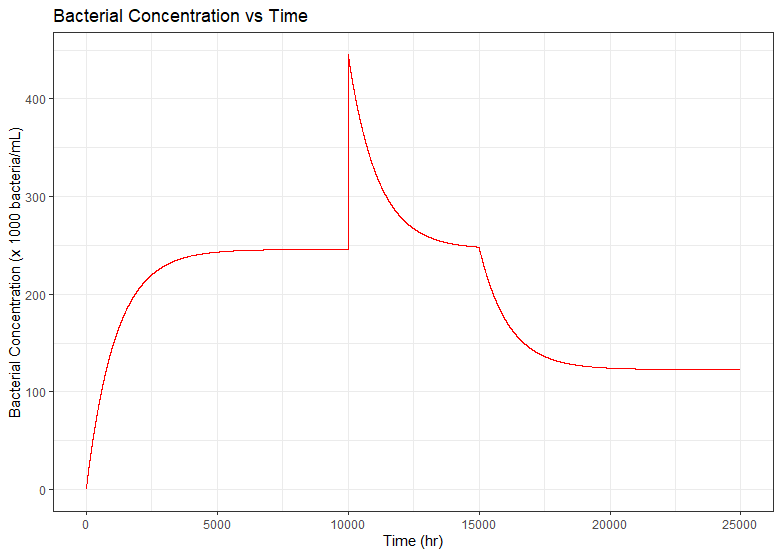
\includegraphics[scale=0.5]{plots/NoPhage_U_perturbed_down.png}

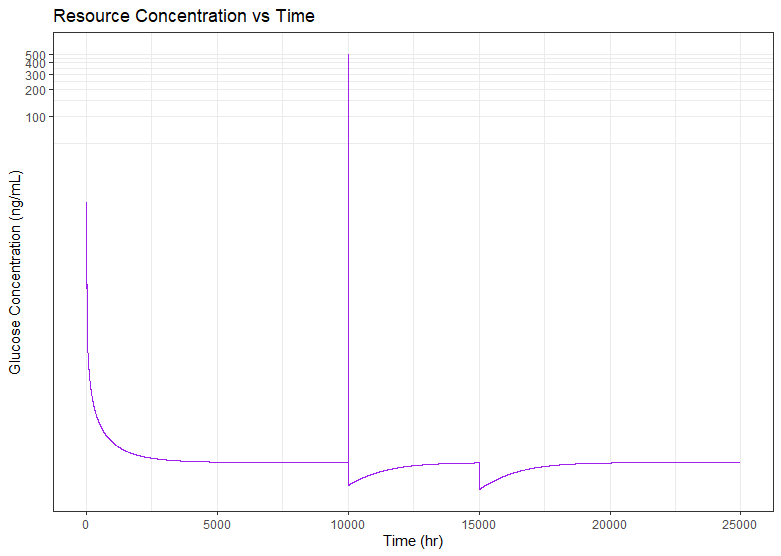
\includegraphics[scale=0.5]{plots/NoPhage_R_perturbed_down.png}
\end{center}

In this last example, I have decreased the infusion rate to half of its original amount at t=15000. According to the equilibrium equations, this change should decrease the carrying capacity by half and should not change the equilibrium resource concentration. Both changes are reflected in these plots.

\subsection {Bacteria with phage - Basic model}
\subsubsection{Lysogen Takeover}

\begin{center}
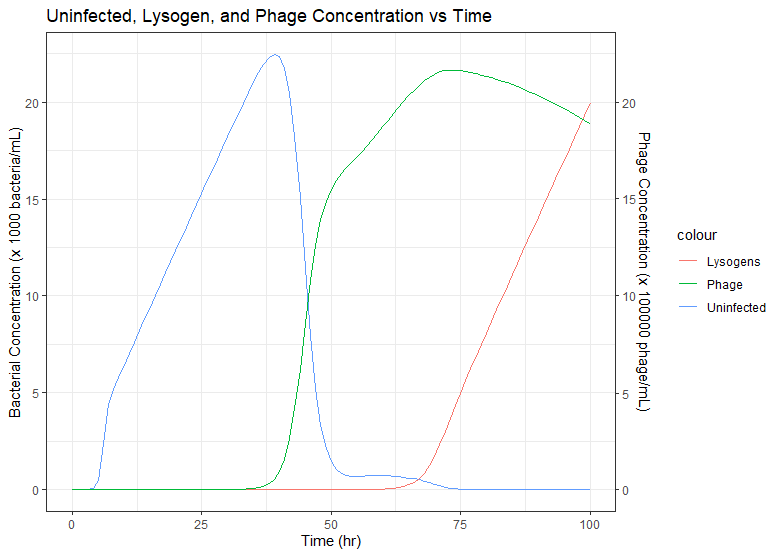
\includegraphics[scale=0.5]{plots/Basic_U_L_P.png}
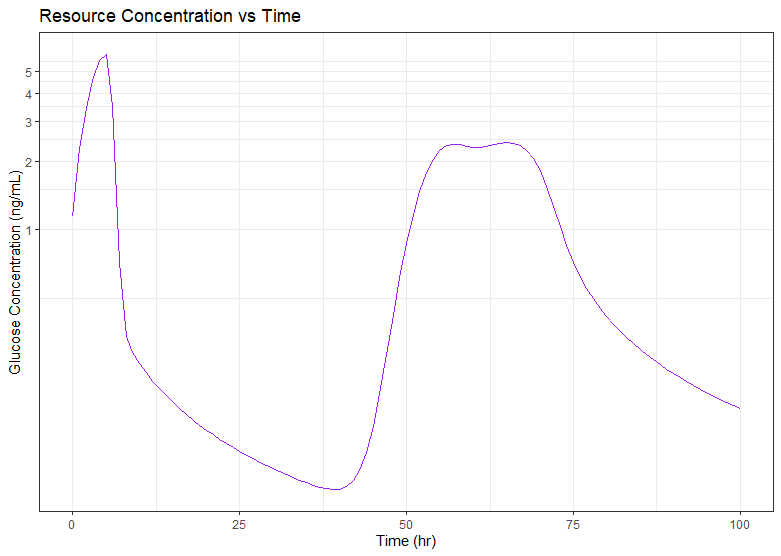
\includegraphics[scale=0.5]{plots/Basic_R.png}
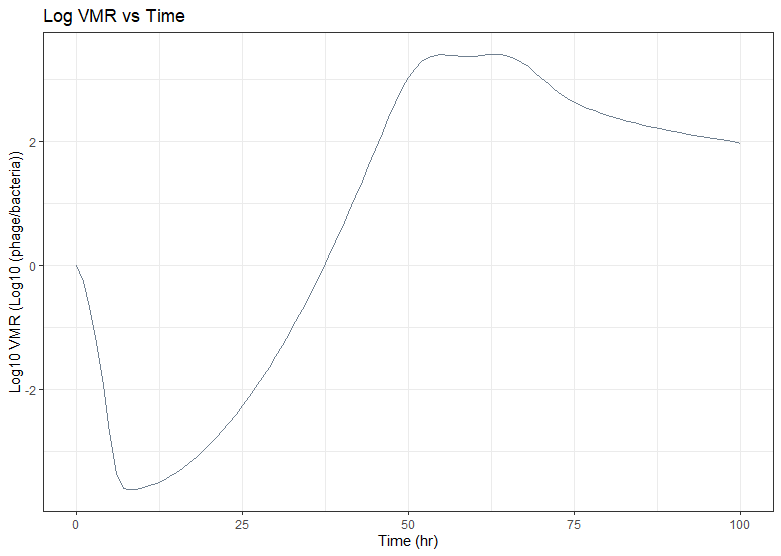
\includegraphics[scale=0.5]{plots/Basic_VMR.png}
\end{center}

These plots are representative of the early course of a typical infection (where lysogens take over the population). In the early stages (roughly t=0-25 hours), phage concentrations are low, and therefore the population of uninfected bacteria grows according to the dynamics discussed previously. During this time, the bacterial concentration increases more quickly than the phage concentration, and decreases significantly below 1 (the VMR in this plot starts at 1; the VMR is the viral-microbe ratio, the ratio of free phage to bacteria). 

At some point (roughly t=40), the phage concentration starts increasing rapidly, leading to the suppression of uninfected growth. (Notice that in the first plot, the phage scale is 100x This leads to a quick rise in the number of phages, which then lead to the killing or lysogenization of a significant portion of the uninfected population. In this case, since the probability of lysogeny is low, most of the uninfected population is killed, leading to a high VMR (in this case, on the order of $10^{2.5}$). While most of the bacteria are killed, a second peak in resource concentration begins due to low resource utilization. Finally, lysogens dominate the bacterial population (as they are not killed by the free phages). 

\subsubsection{Population equilibrium}

\begin{center}
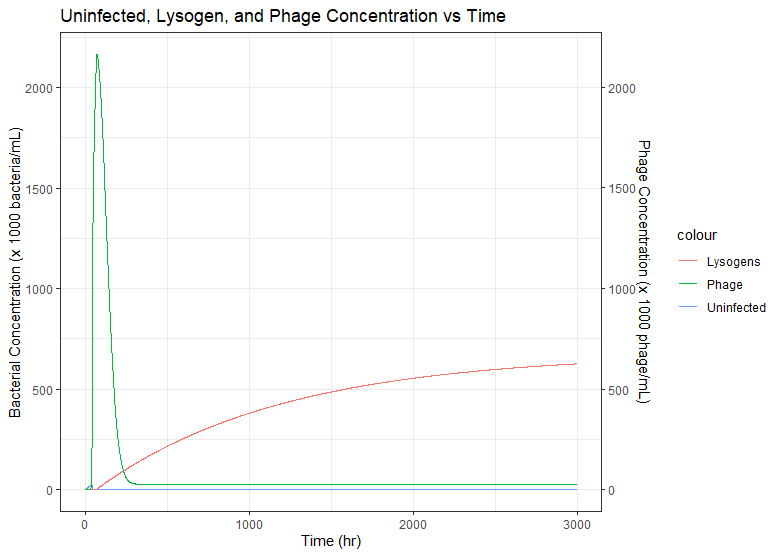
\includegraphics[scale=0.5]{plots/Basic_U_L_P_unzoomed.png}

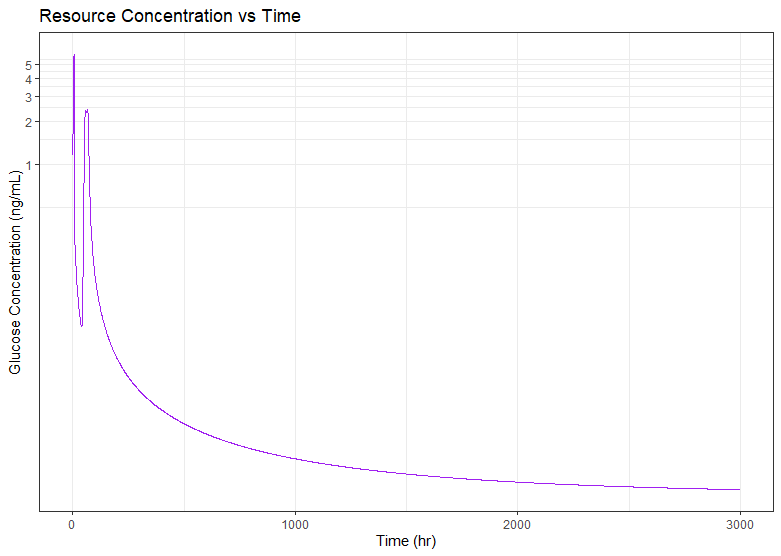
\includegraphics[scale=0.5]{plots/Basic_R_unzoomed.png}

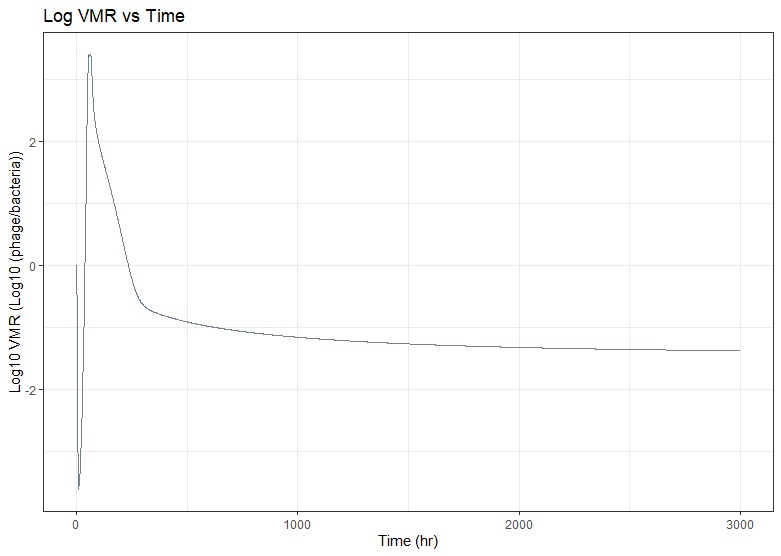
\includegraphics[scale=0.5]{plots/Basic_VMR_unzoomed.png}
\end{center}

As there exist few uninfected bacteria in the population after the lysogen takeover, the phage population decreases due to adsorbing to phages. At equilibrium, the free phage concentration is relatively low and maintained by induction from lysogens. The final equilibrium VMR with these parameters is about $10^{-1.5}$, which is fairly low compared to other models (Weitz et al., 2017). However, it is important to note that the VMR may vary widely based on the parameter choices. Additionally, in an actual ecosystem, there would likely be multiple species of phages, some of which may be virulent phages, which could predate upon a single bacterial species, which may increase the observed VMR. From the section 5 analyses, 

\begin{center}$
\text{VMR} = \frac{\beta r e (D_B + r)}{K_a i + D_pe (D_B + r)}$
\end{center}
meaning that the VMR is approximately linear with respect to r, which I estimate can span multiple orders of magnitude depending on conditions. Additionally, the VMR further depends on $K_a$, which also may span multiple orders of magnitude. While most of the simulations observed showed VMRs less than 1, VMRs greater than 1 have been observed.

How accurate were the predictions in this case?

There are essentially 0 uninfected bacteria at equilibrium, as predicted. The estimated phage concentration of 26582.56 phages/mL was the same as the actual phage concentration, while the estimated lysogen concentration was significantly lower than the actual phage concentration (549288.4 estimated vs 625991.1 actual bacteria/mL). The resource concentration was slightly lower than predicted ($5.85 \times 10^{-12}$ estimated vs $5.14 \times 10^{-12}$ actual), although these errors were all in the expected direction. The predicted VMR of 0.048 was similar to the actual VMR of 0.042, which is likely because both lysogen predictions and phage predictions are relatively close to their actual value.

\subsection{Bacteria with phage - multiplicity of infection model}

\begin{center}
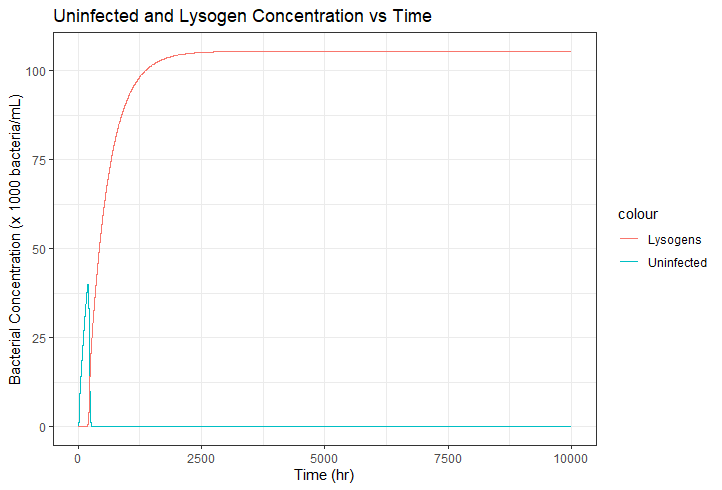
\includegraphics[scale=0.5]{plots/MOI_U_L.png}

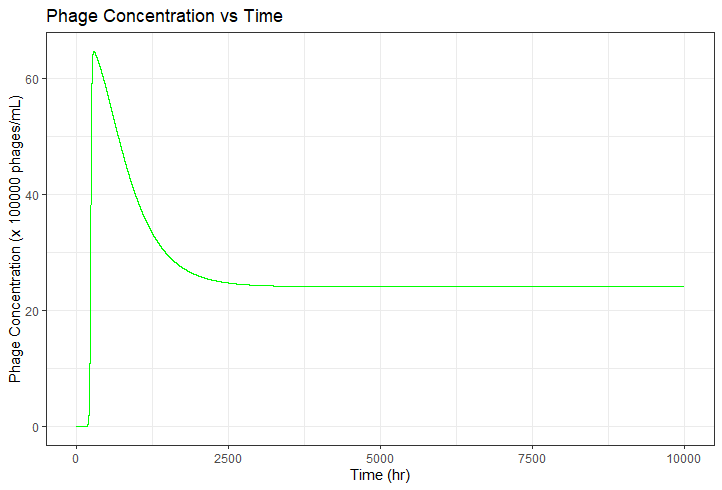
\includegraphics[scale=0.5]{plots/MOI_P.png}

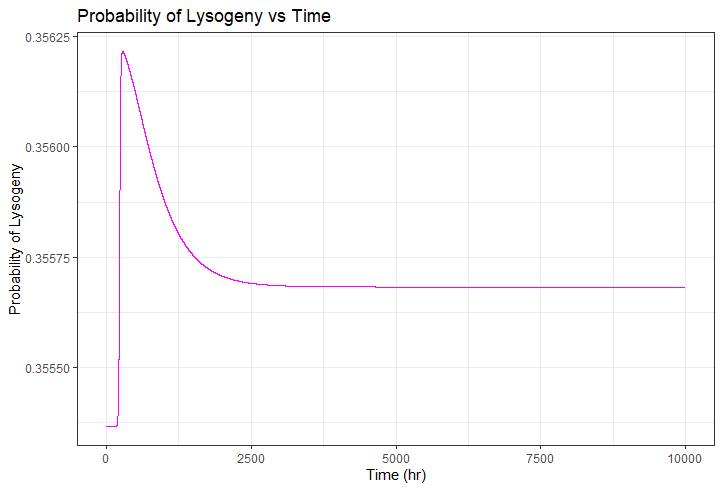
\includegraphics[scale=0.5]{plots/MOI_phi.png}
\end{center}

I don't include all the plots here because the results are essentially the same as the basic model. (As another example of the equilibrium VMR, this VMR is about 20, but that does not have do do with the adaptation of $\phi$.)

The reason why the results for this model are similar to the basic model are because the probability of lysogeny varies so little with respect to the phage concentration; with 0 phages, the probability of lysogeny from this model is slightly above 0.355; increasing the phage concentration drastically to over 6,000,000 phages/mL only increases the probability of lysogeny by about 0.01. It is likely that the majority of infections at any time point with the conditions possible in this system involve only 1 coinfecting phage, but perhaps it is possible in other systems to have significant differences in the probability of lysogeny due to coinfections. For example, if $10^8$ bacteria/mL (approximately the concentration of stationary phase bacteria) were infected in a laboratory setting with $10^9$ phages/mL, a significant increase in $\phi$ to 0.49 would be predicted, given the $K_a$ in this system (Tsui $\&$ Mark, 1976). 

\section{Notes}
The majority of the code for this project was written in R. The differentials were numerically integrated using deSolve, and the results were plotted using ggplot. The value for K was determined through curve-fitting using the SciPy library in Python. Equilibrium estimates were generated using Maple (see Maple worksheet). Code for the project (which includes the parameters used to generate the representative plots and the parameter estimate of the Hill function) can be found here. \url{https://github.com/Apeirogons/3BM6-Modelling/tree/master/temperate_phage_modelling/scripts}. 

\section{References}

\begin{enumerate}
\item	Allen, R., & Waclaw, B. (2018). Bacterial growth: a statistical physicist’s guide. Reports On Progress In Physics, 82(1), 016601.
\url{https://doi.org/10.1088/1361-6633/aae546}

\item	Cunningham, A., Lennox, J., & Ross, R. (2010). Microbial Growth. Cs.montana.edu. Retrieved 7 April 2020, from \url{https://www.cs.montana.edu/webworks/projects/stevesbook/contents/chapters/chapter002/section002/black/page001.html}.

\item	Delbrück M. (1945). The Burst Size Distribution in the Growth of Bacterial Viruses (Bacteriophages). Journal of bacteriology, 50(2), 131–135. 

\item	Erez, Z., Steinberger-Levy, I., Shamir, M., Doron, S., Stokar-Avihail, A., & Peleg, Y. et al. (2017). Communication between viruses guides lysis–lysogeny decisions. Nature, 541(7638), 488-493. \url{https://doi.org/10.1038/nature21049}

\item	Figliozzi, R., Chen, F., Chi, A., & Hsia, S. (2016). Using the inverse Poisson distribution to calculate multiplicity of infection and viral replication by a high-throughput fluorescent imaging system. Virologica Sinica, 31(2), 180-183. \url{https://doi.org/10.1007/s12250-015-3662-8} 

\item	Füchslin, H., Schneider, C., & Egli, T. (2011). In glucose-limited continuous culture the minimum substrate concentration for growth, smin, is crucial in the competition between the enterobacterium Escherichia coli and Chelatobacter heintzii, an environmentally abundant bacterium. The ISME Journal, 6(4), 777-789. \url{https://doi.org/10.1038/ismej.2011.143}

\item	Gallet, R., Shao, Y., & Wang, I. (2009). High adsorption rate is detrimental to bacteriophage fitness in a biofilm-like environment. BMC Evolutionary Biology, 9(1), 241. \url{https://doi.org/10.1186/1471-2148-9-241} 

\item	Gandon, S. (2016). Why Be Temperate: Lessons from Bacteriophage λ. Trends In Microbiology, 24(5), 356-365. \url{https://doi.org/10.1016/j.tim.2016.02.008}

\item	Hanson, R., & Snyder, J. (1979). Enzymatic determination of glucose in marine environments: Improvement and note of caution. Marine Chemistry, 7(4), 353-362. \url{https://doi.org/10.1016/0304-4203(79)90021-5} 

\item	Mitarai, N., Brown, S., & Sneppen, K. (2016). Population Dynamics of Phage and Bacteria in Spatially Structured Habitats Using Phage λ and Escherichia coli. Journal Of Bacteriology, 198(12), 1783-1793. \url{https://doi.org/10.1128/jb.00965-15}

\item	Phillips, R., & Milo, R. (2009). A feeling for the numbers in biology. Proceedings Of The National Academy Of Sciences, 106(51), 21465-21471. \url{https://doi.org/10.1073/pnas.0907732106}

\item	Ryan, G., & Rutenberg, A. (2007). Clocking Out: Modeling Phage-Induced Lysis of Escherichia coli. Journal Of Bacteriology, 189(13), 4749-4755. \url{https://doi.org/10.1128/jb.00392-07}

\item	Sinha, V., Goyal, A., Svenningsen, S., Semsey, S., & Krishna, S. (2017). In silico Evolution of Lysis-Lysogeny Strategies Reproduces Observed Lysogeny Propensities in Temperate Bacteriophages. Frontiers In Microbiology, 8. \url{https://doi.org/10.3389/fmicb.2017.01386}

\item	Storms, Z., & Sauvageau, D. (2015). Modeling tailed bacteriophage adsorption: Insight into mechanisms. Virology, 485, 355-362.
\url{https://doi.org/10.1016/j.virol.2015.08.007}

\item	Tsui, L., & Mark, K. (1976). The depression of endolysin synthesis in bacteria infected with high multiplicities of phage λ. Molecular And General Genetics MGG, 143(3), 269-278. \url{https://doi.org/10.1007/bf00269403}

\item	Weitz, J., Beckett, S., Brum, J., Cael, B., & Dushoff, J. (2017). Lysis, lysogeny and virus–microbe ratios. Nature, 549(7672), E1-E3. \url{https://doi.org/10.1038/nature23295}

\item	Zeng, L., Skinner, S., Zong, C., Sippy, J., Feiss, M., & Golding, I. (2010). Decision Making at a Subcellular Level Determines the Outcome of Bacteriophage Infection. Cell, 141(4), 682-691. \url{https://doi.org/10.1016/j.cell.2010.03.034}

\item	Ziv, N., Brandt, N., & Gresham, D. (2013). The Use of Chemostats in Microbial Systems Biology. Journal Of Visualized Experiments, (80). \url{https://doi.org/10.3791/50168}
\end{enumerate}
\end{section}

\end{document}


